\chapter{Eredmények}
\pagestyle{headings}

\section{Grafit-modell}
\subsection{Potenciáltérképezések}
Mint korábban említettem már, a pásztázó elektrokémiai mikroszkópiában általában egy céltárgy felszínét vizsgáljuk vagy az azon lejátszódó folyamatról szeretnénk információhoz jutni. Először egy jól ismert rendszert vizsgáltam meg, az előzőekben részletesebben jellemzett grafit elektródpárt. A céltárgyat 2000 mV-al pozítivan polarizáltam, katódosan és anódosan egymáshoz képest. A pásztázási terület horizontális esetben 4000x3000 $\upmu$m volt az X-Y síkon, és Z irányban 200 $\upmu$m-el toltam el a két mérés között. Vertikális pásztázás esetén 5000x1000 $\upmu$m volt az X-Z síkon a vizsgált terület. A feltérképezett katód környezetében hidrogén-ion redukciójára, az anódos oldalon pedig oxigén gáz fejlődésre számíthatunk, a következő egyenletek szerint:

K(-): 2H$^+$ + 2e$^-$ $\longrightarrow$ H$_2$ (redukció)

A(+):  2OH$^-$ $\longrightarrow$ 0,5 O$_2$ + H$_2$O + 2e$^-$ (oxidáció)

A mikroméretű referenciaelektróddal készített pásztázások horizontális potenciáltérképeit a (\ref{fig:horizontális}. ábra E,F), a vertikálisat pedig az (\ref{fig:vertikális}. ábra C) láthatjuk. A várakozásnak megfelelő eredményeket kaptam, hiszen mind a vertikális mind pedig a horizontális képeken, -5 mV eltéréssel, azonos potenciáltartományba esnek a mérések eredményei. Továbbá jól látható, hogy az elektródpár tagjai a polarizáció hatására katódként (-295 mV körüli átlagérték) és anódként (-265 mV körüli átlagérték) viselkedtek, ahogy arra számítottunk. Így az eredményekből látható, hogy a tanulmányozott rendszer ténylegesen állandó, jól jellemezhető és ez a módszer alkalmazható a potenciáltérképezésre. 

\subsection{Elektromos mező és az áramsűrűség}
A \emph{Módszerek} című fejezetben említettek szerint elvégeztem a számolásokat, deriválást és így ábrázoltam vektorosan az elektromos mezőt, ami a (\ref{fig:field_h}. ábra C), (\ref{fig:field_h1}. ábra C) és az (\ref{fig:field_v}. ábra C) láthatóak a grafit céltárgy esetében. Ezen belül az (\ref{fig:field_h}. ábra C) és (\ref{fig:field_h1}. ábra C) a horizontális pásztázások eredményei, az (\ref{fig:field_v}. ábra C) képe pedig a vertikális. A Z tengelyen nézve az anód esetében az áramvektorok az oxidáció következtében a síkből kifelé mutatnak, a katódnál a redukció miatt pedig a síkba mutatnak a vektorok. Az X-Y síkon pedig az anódból a katód felé irányulnak a vetorok.  

Hasonlóan, az előző fejezetben leírtak alapján, elkészítettem az áramsűrűség térképét a Z irányú komponens szerint, a horizontális pásztázásra. Szakirodalomak alapján elmondhatjuk, hogy az anódos áramsűrűség pozitív értéket, a katódos pedig negatívat ad \cite{bastos2016preliminary}. Jól látható az (\ref{fig:áramsűrűség}. ábra C) képen, hogy a katód helyén (piros színnel jelölt) és környezetében negatív értékeket kaptam, az anód esetében (kék színnel jelölt) pedig pozitív értékeket, ahogy vártuk. A zölddel jelölt részen körülbelül 0-nak tekinthető az áramerősség. Továbbá megfigyelhetjuk, hogy körülbelül szimmetrikusnak mondható a katód és anód régiójában áramerősség és ez távolódva a helyüktől csökkenést mutat. Ez a térkép az elektromos mezőével mutat hasonlóságot, mivel az előzőleg már említett (\ref{fig:nabla}. egyenlet) szerint a két érték között egyenes arányosság van \cite{{isaacs1981scanning,bastos2017application}}. Az eredmények a várakozással egyeztek ezen esetben is, így ezt a galvánpár esetében is alkalmaztam.

\section{Vas-cink galvánpár korrózió vizsgálata}
\subsection{Potenciáltérképezések}
Az előző alfejezetben bemutatott grafit céltárgy után egy vas-cink galvánpárból készült céltárgyat tanulmányoztam, melyet a \emph{Módszerek} fejezetben jellemeztem részletesebben. A pásztázási terület az anód és katód esetében is 3000x2000 volt az X-Y síkon, horizontális mérések esetén, és 400 $\upmu$m a Z irányú eltolás. Vertikális mérések során ez 3000x1000 $\upmu$m volt az X-Z síkon. Ez egy sokszor vizsgált rendszer, mivel a vas ötvözeteit, illetve magát a vasat is, számos esetben vonjuk be a jobb korrózióállóság miatt cinkréteggel. Ezt a technikát a hétköznapi életben horganyzásnak hívjuk, ezzel a módszerrel jelentős mértékben csökkenthető a védett fém korróziója. Ez annak tulajdonítható, hogy a cink tölti be az \emph{Irodalom} fejezetben említett áldozati anód szerepét a galvanikus kapcsolat során. Tehát a cink oxidálódik a védett fém, vagyis a vas helyett. Ezzel egyidőben a vason redukció zajlik, viszont vaskioldódás nélkül. A cella szétkapcsolása esetén, lokális anód és katód alakulna ki a vas felületén. Elvesztené a cink anódos védelmét és elindulna a rozsdásodás folyamata.
A védett vason végbemenő folyamatnak is a lényege a hidrogén-ion redukció, ahogy az előző alfejezetben jellemzett grafit katód esetén is: 

2H$^+$ + 2e$^-$ $\longrightarrow$ H$_2$

O$_2$ + 4H$_2$O + 4e$^-$ $\longrightarrow$ 2H$_2$O + 4OH$^-$

A cink anódon a következő reakciók játszódnak le:

2 Zn $\longrightarrow$ 2 Zn$^{2+}$ + 4e$^-$ 

Zn$^{2+}$ + nH$_2$O $\longrightarrow$ Zn(OH)$_{n2-n}$ + nH$^+$

A vizsgálatok potenciáltérképei az (\ref{fig:horizontális}. ábra) és (\ref{fig:vertikális}. ábra) láthatóak. Ebben az esetben külön pásztáztam, a katód (\ref{fig:horizontális}. ábra A,B) és az anód (\ref{fig:horizontális}. ábra C,D) felületét a grafittal ellentétben. A felület homogén, vagyis a vas egész felülete katódként viselkedett a cellában a mérés alatt, ezzel alátámasztva, hogy a cinkelektród működött csak anódként. Ezt bizonyítja az eltérő mért potenciálértékek is, vagyis anódra jellemzően nagyobb (-230 mV körüli) érték, és a katód esetében kisebb (-275 mV körüli) érték. Illetve leolvasható, hogy a potenciáltartomány értékei a pásztázásoknak körülbelül azonos minimum és maximum értéket követnek itt is. A vas vertikális potenciálképénél (\ref{fig:vertikális}. ábra A) látható egy szélesebb tartomány, mint a horizontális képeknél. Ez valószínűleg annak tulajdonítható, hogy a grafittól eltérően, ez a korróziós folyamat időben változó. A vertikális pásztázása és a horizontálisak között több idő telhetett el, ami során a reakció előre haladt már, így kaptam az eltérő értékeket a tartományra. 

\subsection{Elektromos mező és az áramsűrűség}

Az előző fejezetben leírtak szerint ábrázoltam vektorosan ebben az esetben is az elektromos mezőt, ami az (\ref{fig:field_h}. ábra A,B), (\ref{fig:field_h1}. ábra A,B) és az (\ref{fig:field_v}. ábra A,B) láthatóak a vas-cink galvánpár esetében. Ezen belül az (\ref{fig:field_h}. ábra A) és (\ref{fig:field_h1}. ábra A) a vas katód, ((\ref{fig:field_h}. ábra B) és (\ref{fig:field_h1}. ábra B) a cink anód horizontális pásztázásainak eredményei, az (\ref{fig:field_v}. ábra A) képe a vas katód, (\ref{fig:field_v}. ábra B) képe pedig a cink anód a vertikális eredményei. A Z tengely szerint nézve a vas katód esetében az áramvektorok a síkből kifelé mutatnak, az előző alfejezetben leírtak szerint végbemenő redukció miatt. A cink anódnál pedig, a említett egyenletek szerint lejátszódó oxidáció miatt, a síkba mutatnak a vektorok. Az X-Y síkon is jól látható ez az elv.

Hasonlóan, jártam el a galvánpár esetben is, mikor elkészítettem a horizontális pásztázások áramsűrűség térképét a Z irányú komponens szerint. A grafithoz hasonlóan, az anódos áramsűrűség pozitív értéket, a katódos pedig negatív értéket ad. Megfigyelhető az (\ref{fig:áramsűrűség}. ábra A) képén, hogy az vas katód lokális környezetében negatív értékeket kaptam. Ugyanezen ábra (B) képén a cink anód esetében pedig pozitív értékeket, ahogy vártuk. Ezen céltárgynál is elmondhatjuk, hogy körülbelül szimmetrikus a katód és anód régiójában áramerősség és ez távolódva a helyüktől csökkenést mutat. Illetve a térkép itt is hasonlóságot mutat az elektromos mezőével.

%\includegraphics[trim = 10mm 40mm 0mm 40mm, clip, width=0.4\textwidth, angle=-90]{img/mg_metal/liquid_uncoupled.eps} \includegraphics[trim = 10mm 40mm 0mm 40mm, clip, width=0.4\textwidth, angle=-90]{img/mg_metal/solid_uncoupled.eps}

\begin{figure}
\centering
\includegraphics[width=0.3\textwidth, angle=-90]{img/mérések/Fe_h_100.eps}\includegraphics[width=0.3\textwidth, angle=-90]{img/mérések/Fe_h_500.eps}

\includegraphics[width=0.3\textwidth, angle=-90]{img/mérések/Zn_h_100.eps}\includegraphics[width=0.3\textwidth, angle=-90]{img/mérések/Zn_h_500.eps}

\includegraphics[width=0.3\textwidth, angle=-90]{img/mérések/grafit_h1_100.eps}
\includegraphics[width=0.3\textwidth, angle=-90]{img/mérések/grafit_h_300.eps}

\caption{Az említett céltárgyakról készült horizontális potenciáltérképek:
(A) és (B) a vas katód 100$\upmu$m és 500$\upmu$m magasságban, (C) és (D) a cink anód 100$\upmu$m és 500$\upmu$m magasságban és (E) és (F) a grafit katódja és anódja 100$\upmu$m és 300$\upmu$m magasságban mérve}
\label{fig:horizontális}
\end{figure}


\begin{figure}
\centering
\includegraphics[width=0.3\textwidth, angle=-90]{img/mérések/Fe_v.eps}
\includegraphics[width=0.3\textwidth, angle=-90]{img/mérések/Zn_v.eps}
\includegraphics[width=0.3\textwidth, angle=-90]{img/mérések/grafit_v.eps}


\caption{Az említett céltárgyakról készült vertikális potenciáltérképek:
(A) a vas katód, (B) a cink anód és (C) a grafit katódja és anódja}
\label{fig:vertikális}
\end{figure}

\begin{figure}
\centering
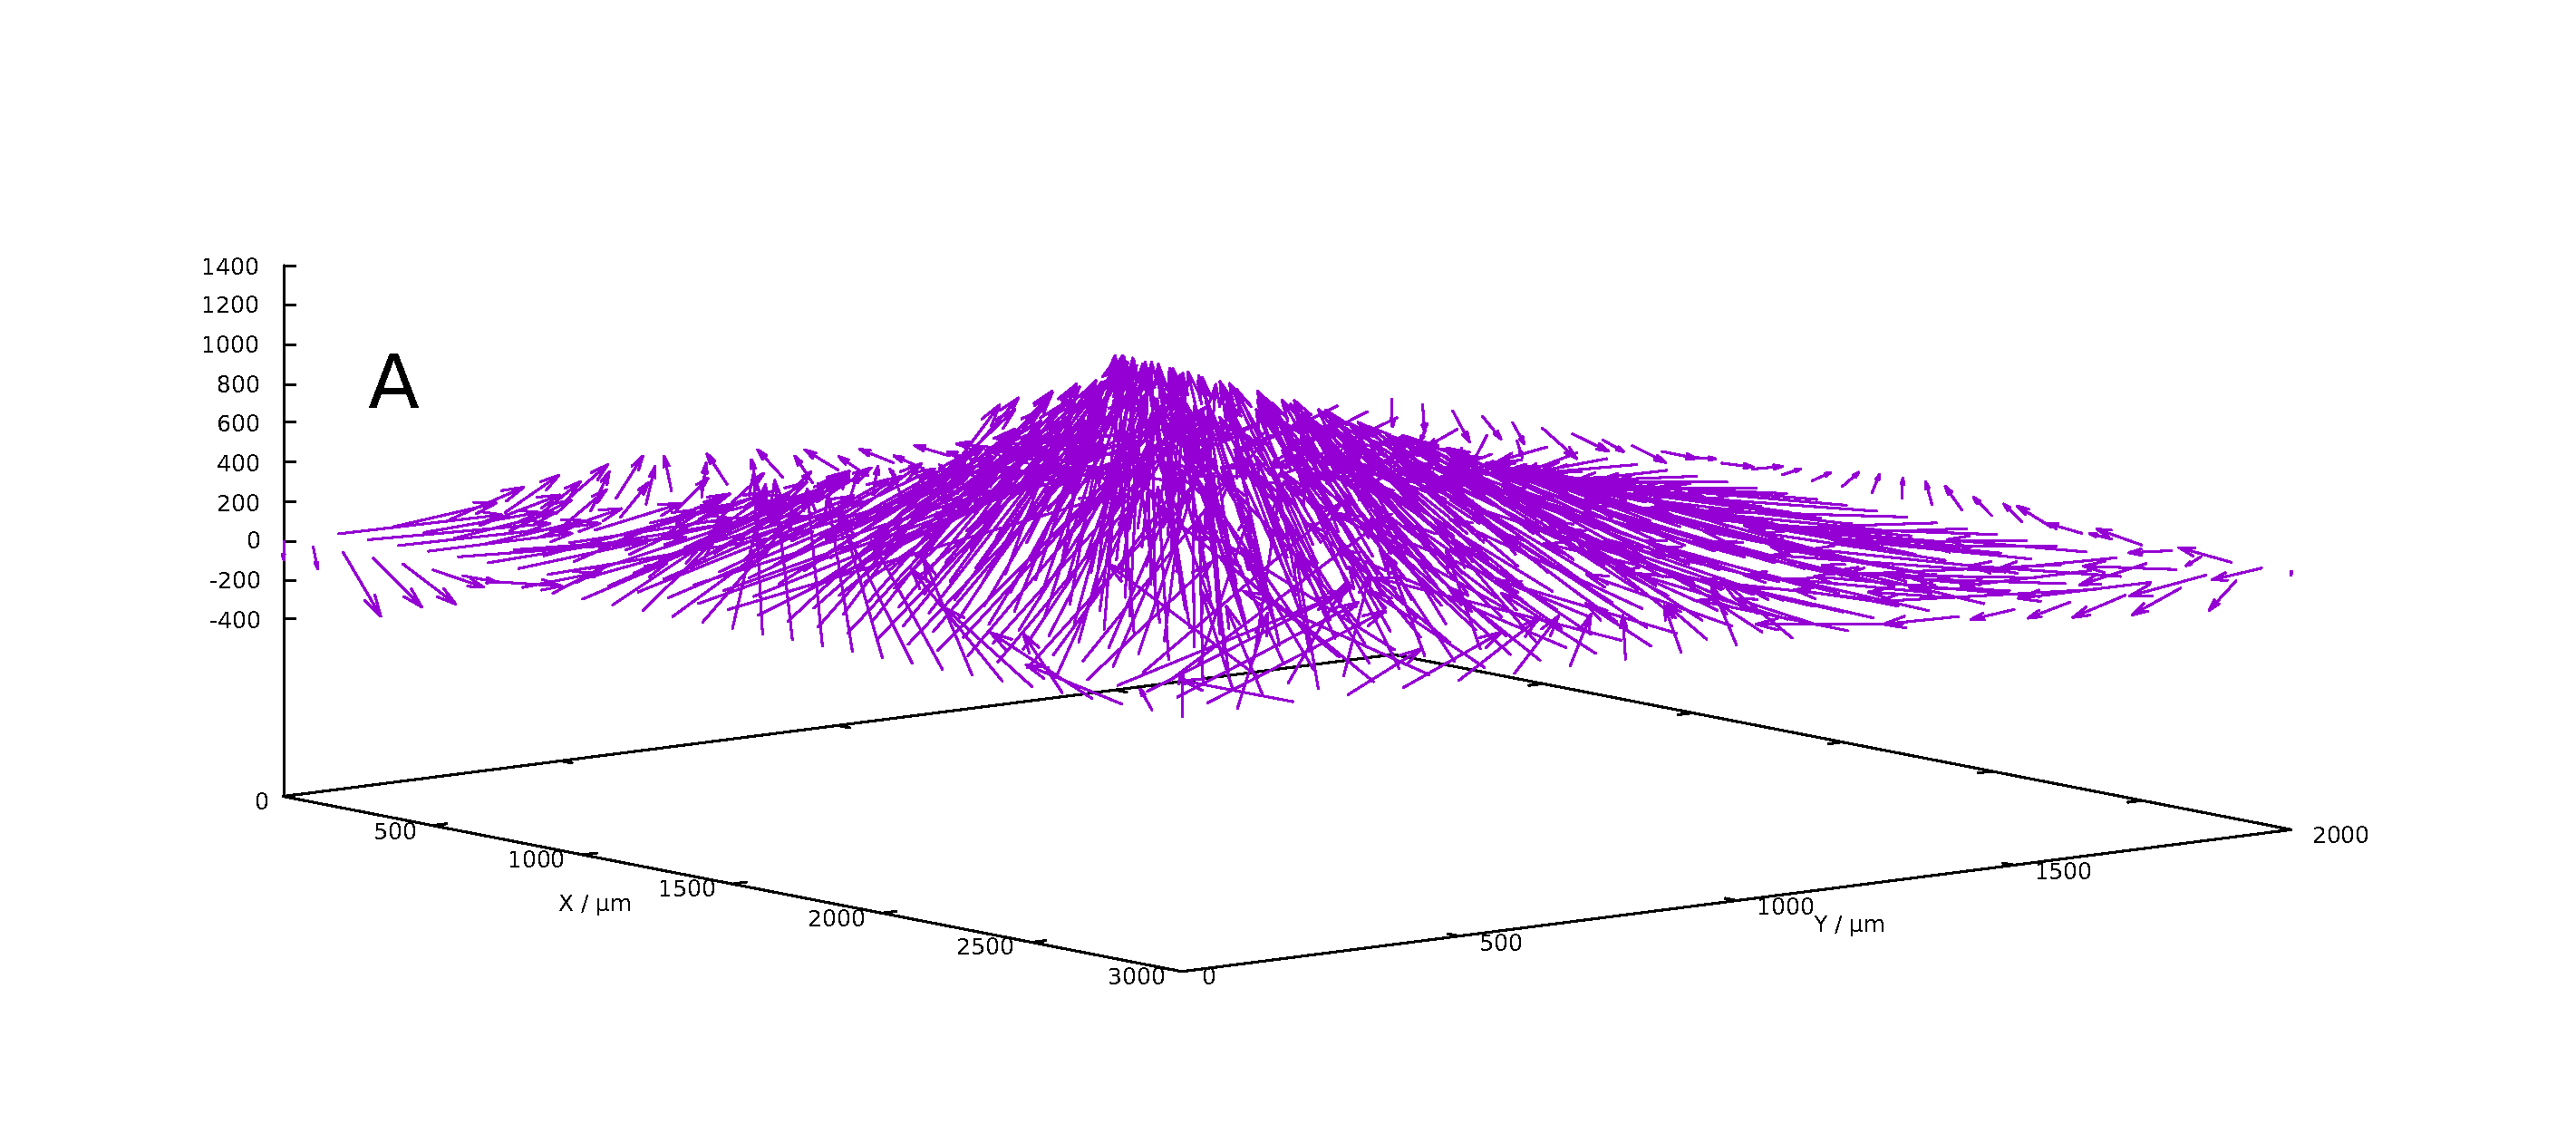
\includegraphics[width=1.2\textwidth]{img/mérések/Fe_h100.pdf}
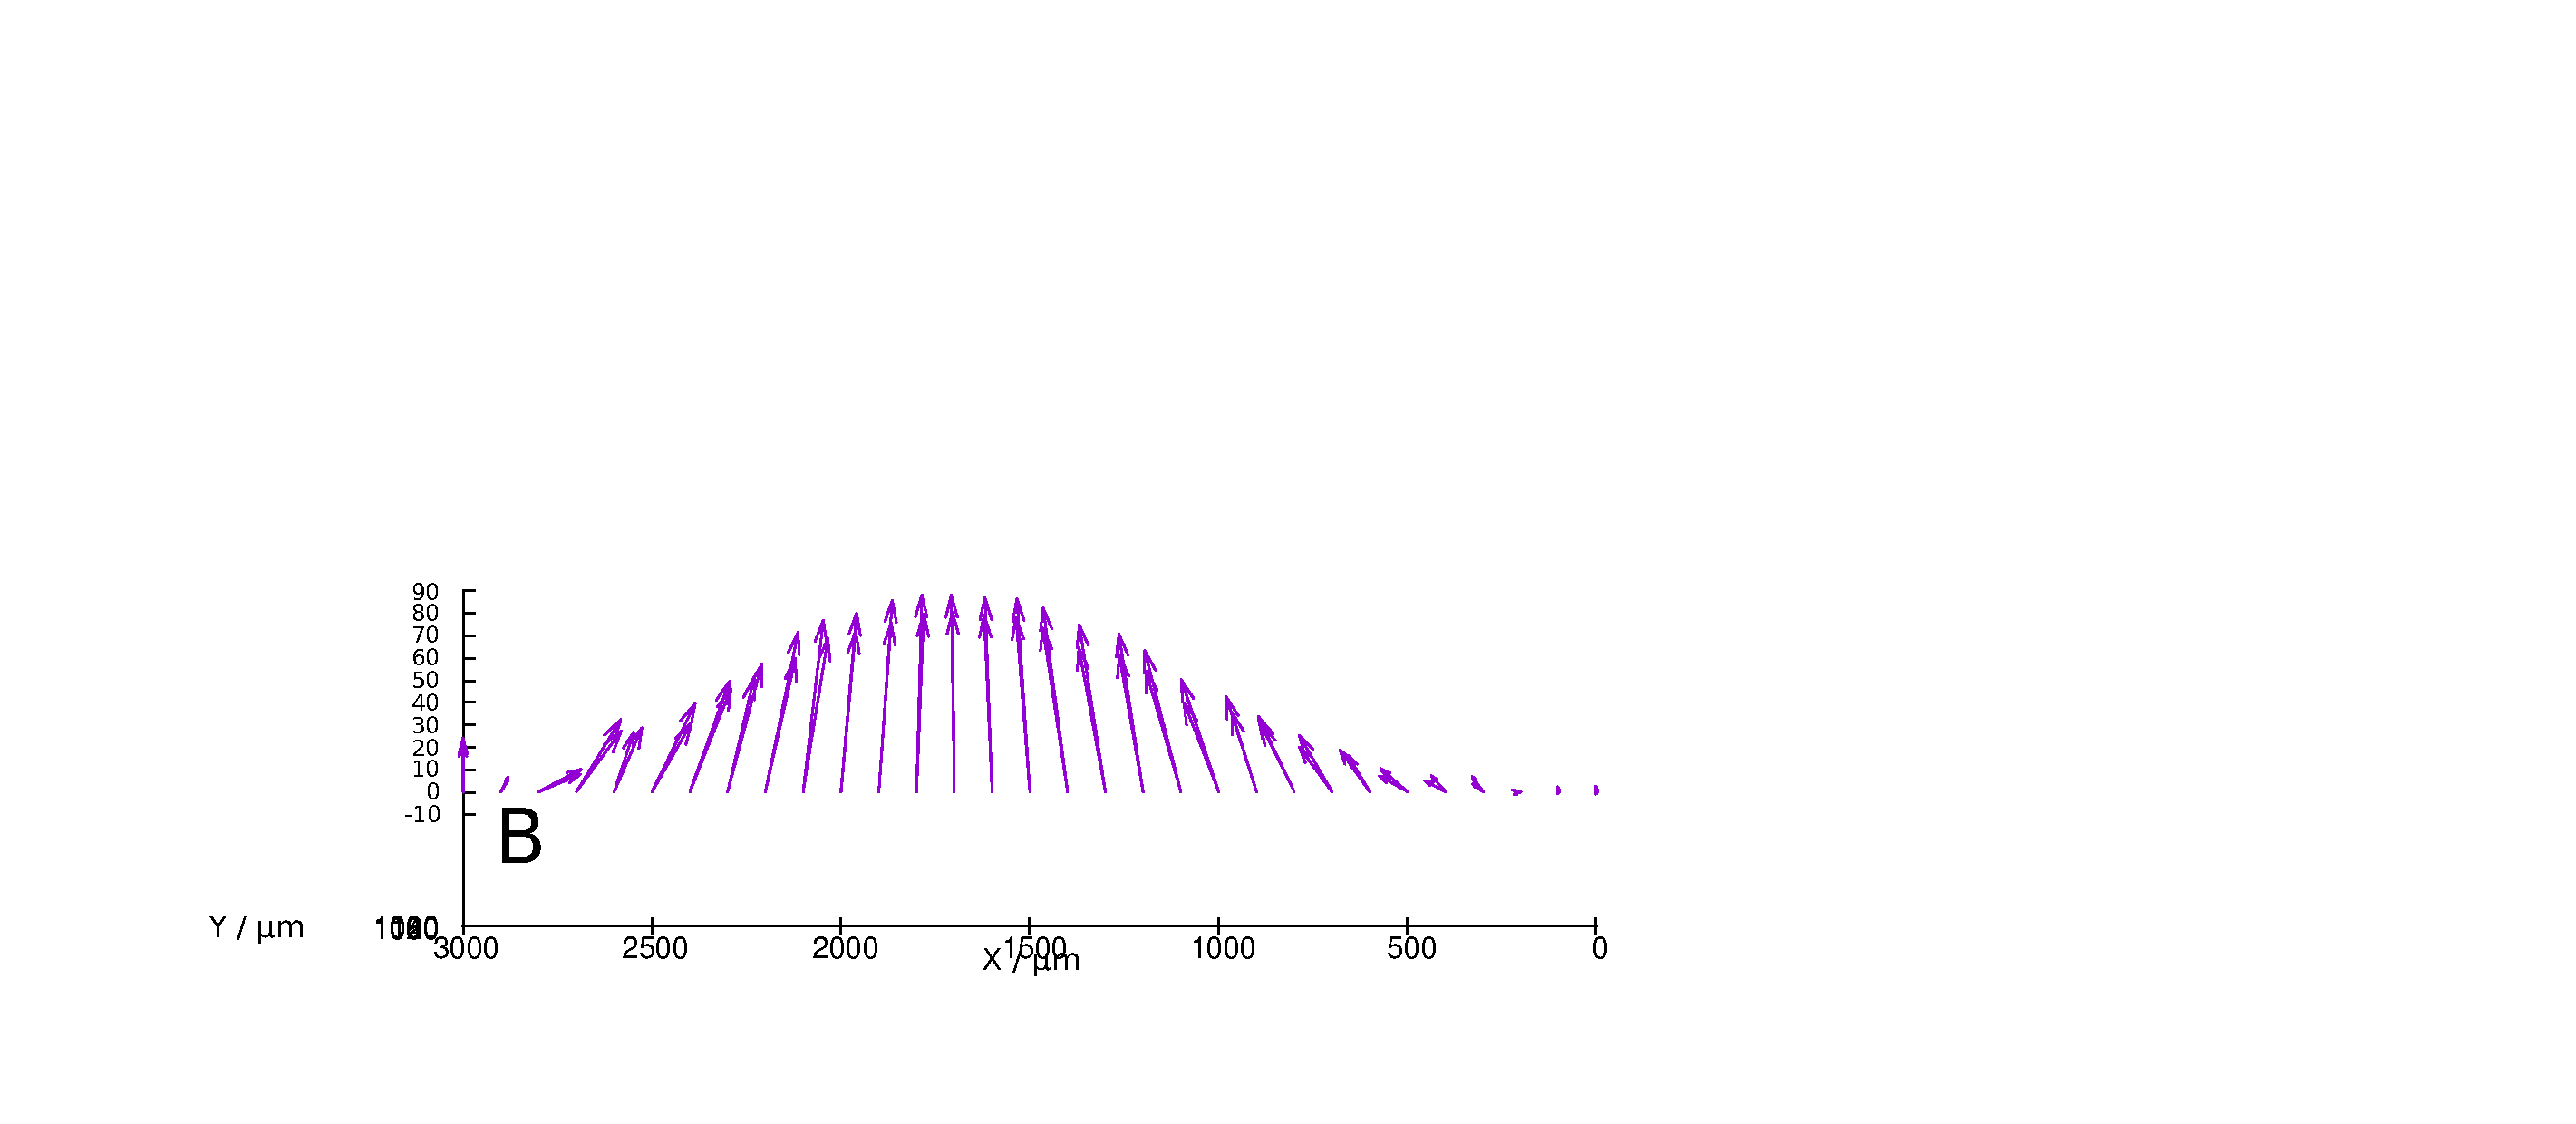
\includegraphics[width=1.2\textwidth]{img/mérések/Zn_h100.pdf}
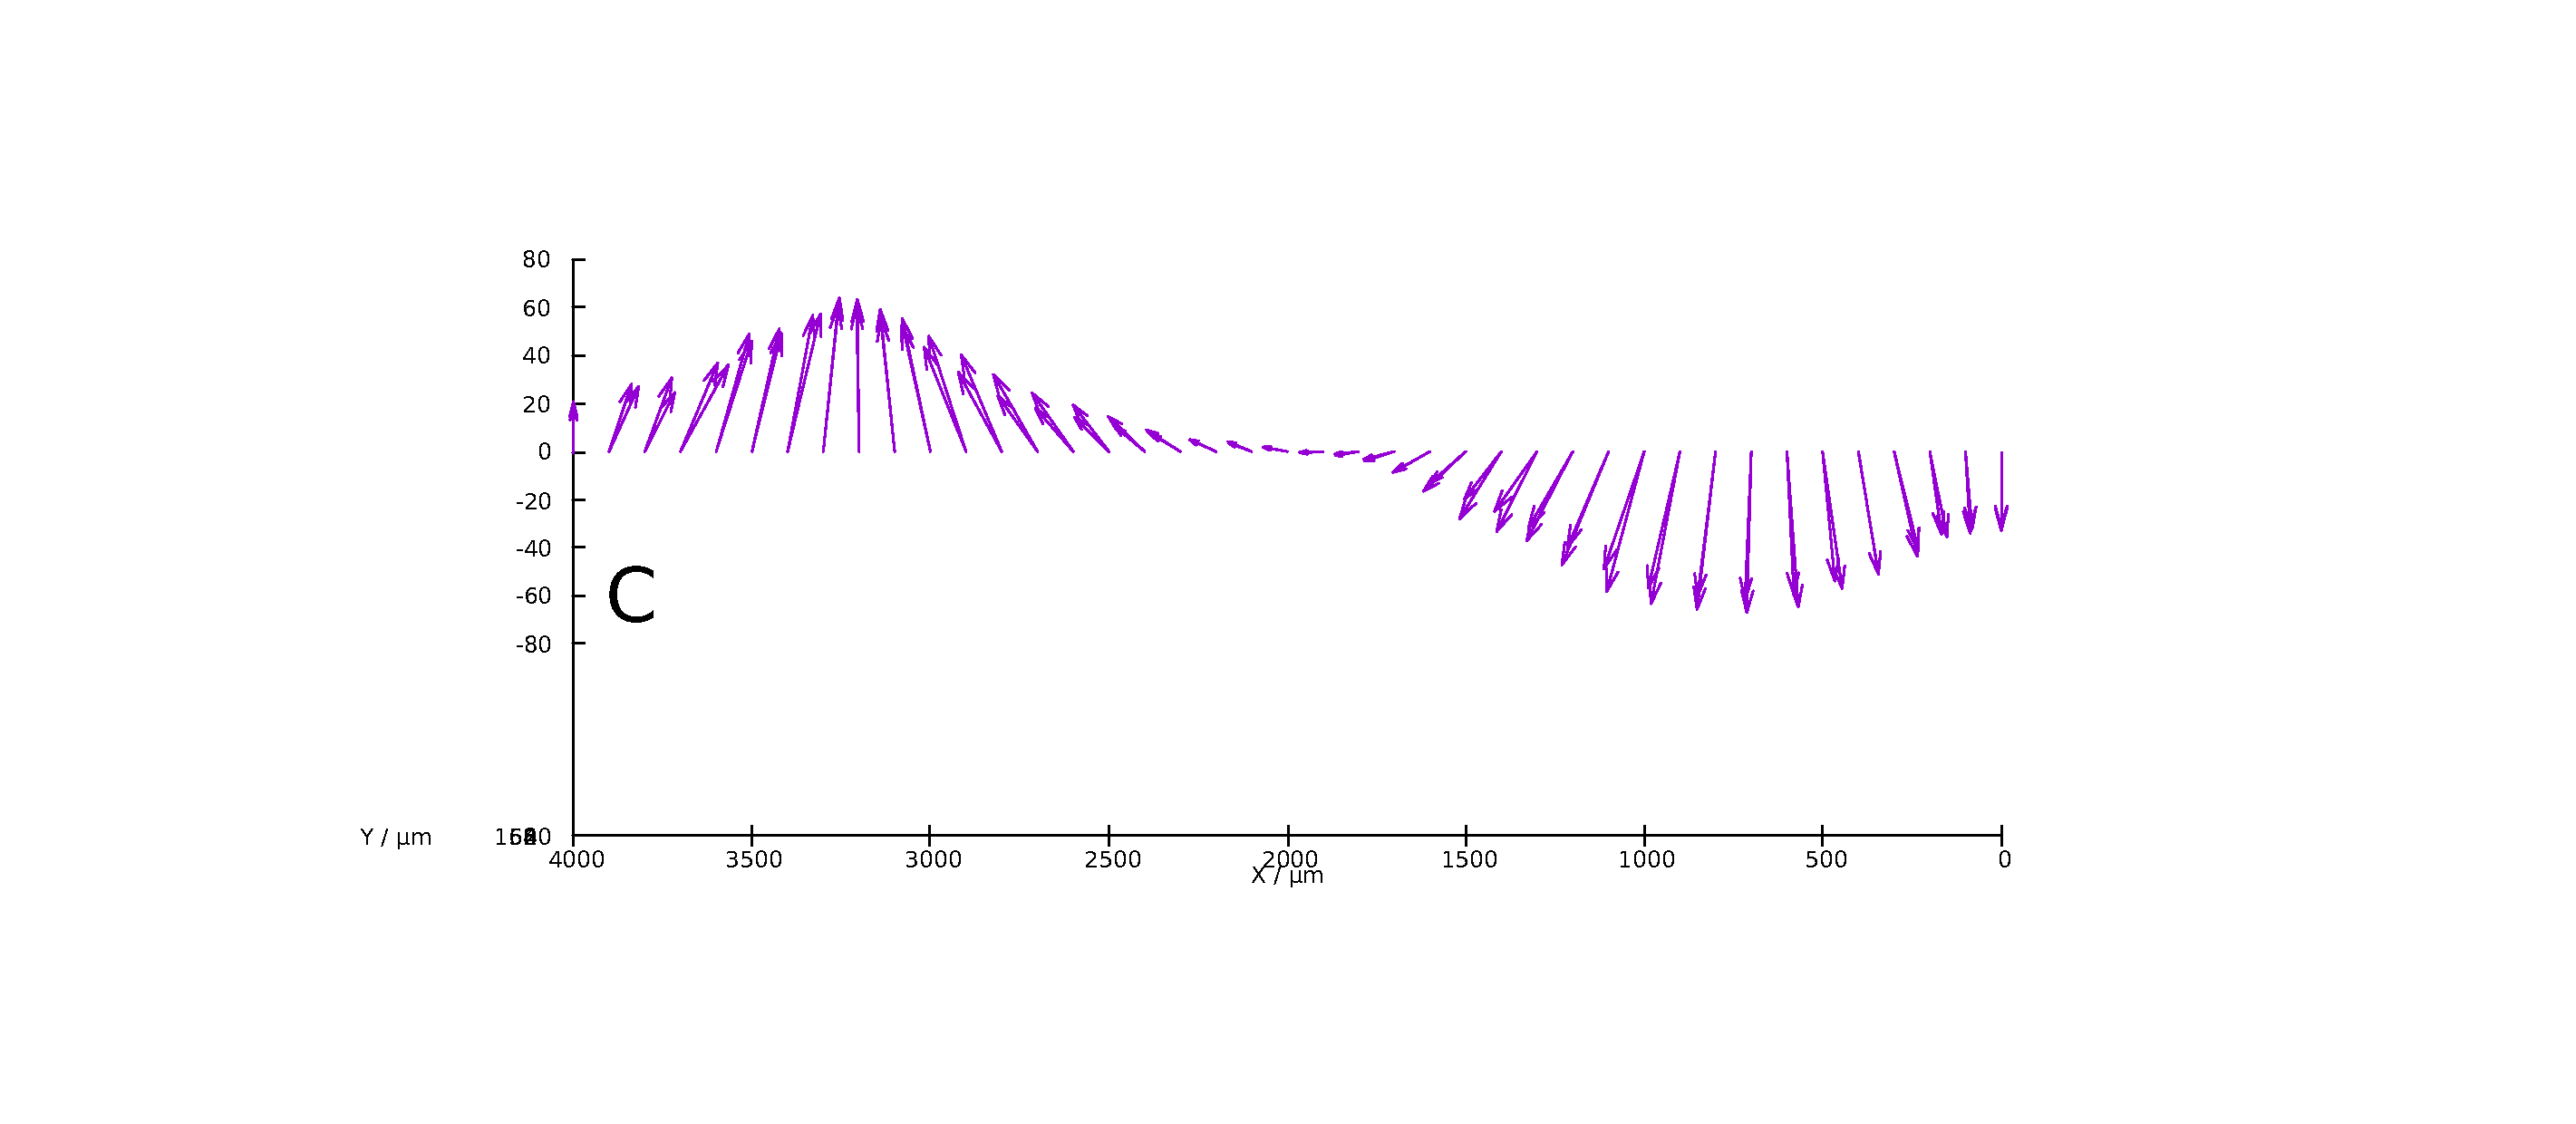
\includegraphics[width=1.2\textwidth]{img/mérések/grafit_h100.pdf}

\caption{Az említett céltárgyakról készült horizontális elektromos mező térképek:
(A) a vas katód, (B) a cink anód és (C) a grafit katódja és anódja 100$\upmu$m magasságban mérve}
\label{fig:field_h}
\end{figure}

\begin{figure}
\centering
\includegraphics[width=0.5\textwidth, angle=-90]{img/mérések/Fe1_h100.eps}
\includegraphics[width=0.5\textwidth, angle=-90]{img/mérések/Zn1_h100.eps}
\includegraphics[width=0.5\textwidth, angle=-90]{img/mérések/grafit1_h100.eps}

\caption{Az említett céltárgyakról készült 2D elektromos mező térképek:
(A) a vas katód, (B) a cink anód és (C) a grafit katódja és anódja 100$\upmu$m magasságban mérve}
\label{fig:field_h1}
\end{figure}

\begin{figure}
\centering
\includegraphics[width=0.4\textwidth, angle=-90]{img/mérések/Fe1_v.eps}
\includegraphics[width=0.4\textwidth, angle=-90]{img/mérések/Zn1_v.eps}
\includegraphics[width=0.4\textwidth, angle=-90]{img/mérések/grafit1_v.eps}

\caption{Az említett céltárgyakról készült vertikális elektromos mező térképek:
(A) a vas katód, (B) a cink anód és (C) a grafit katódja és anódja}
\label{fig:field_v}
\end{figure}

\begin{figure}
\centering
\includegraphics[width=0.5\textwidth, angle=-90]{img/mérések/Fe_h100.eps}
\includegraphics[width=0.5\textwidth, angle=-90]{img/mérések/Zn_h100.eps}
\includegraphics[width=0.5\textwidth, angle=-90]{img/mérések/grafit_h_100.eps}

\caption{Az említett céltárgyakról készült áramsűrűség térképek:
(A) a vas katód, (B) a cink anód és (C) a grafit katódja és anódja}
\label{fig:áramsűrűség}
\end{figure}
